\section{Casi d'uso}
\subsection{Introduzione}
\subsection{Uso della piattaforma da parte di un cliente}
\begin{figure}[H]
    \centering
    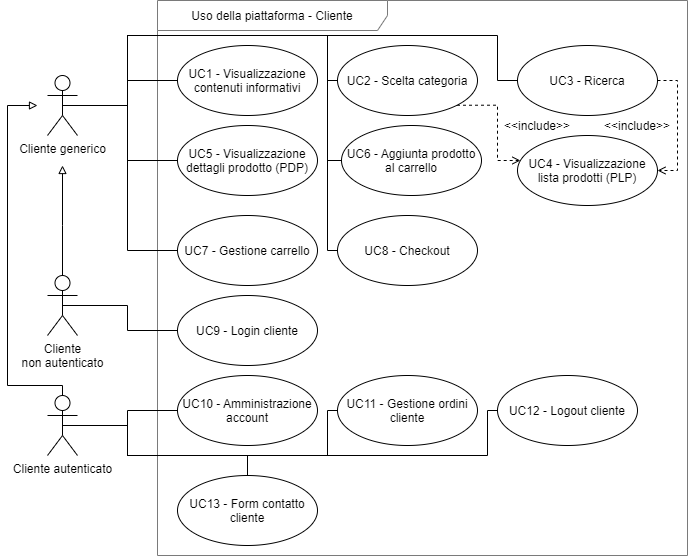
\includegraphics[width=\linewidth]{res/images/UC/cliente.png}
    \caption{Diagramma che descrive le funzionalità della piattaforma} 
\end{figure}
\subsection{Uso della piattaforma da parte di un venditore}
\begin{figure}[H]
    \centering
    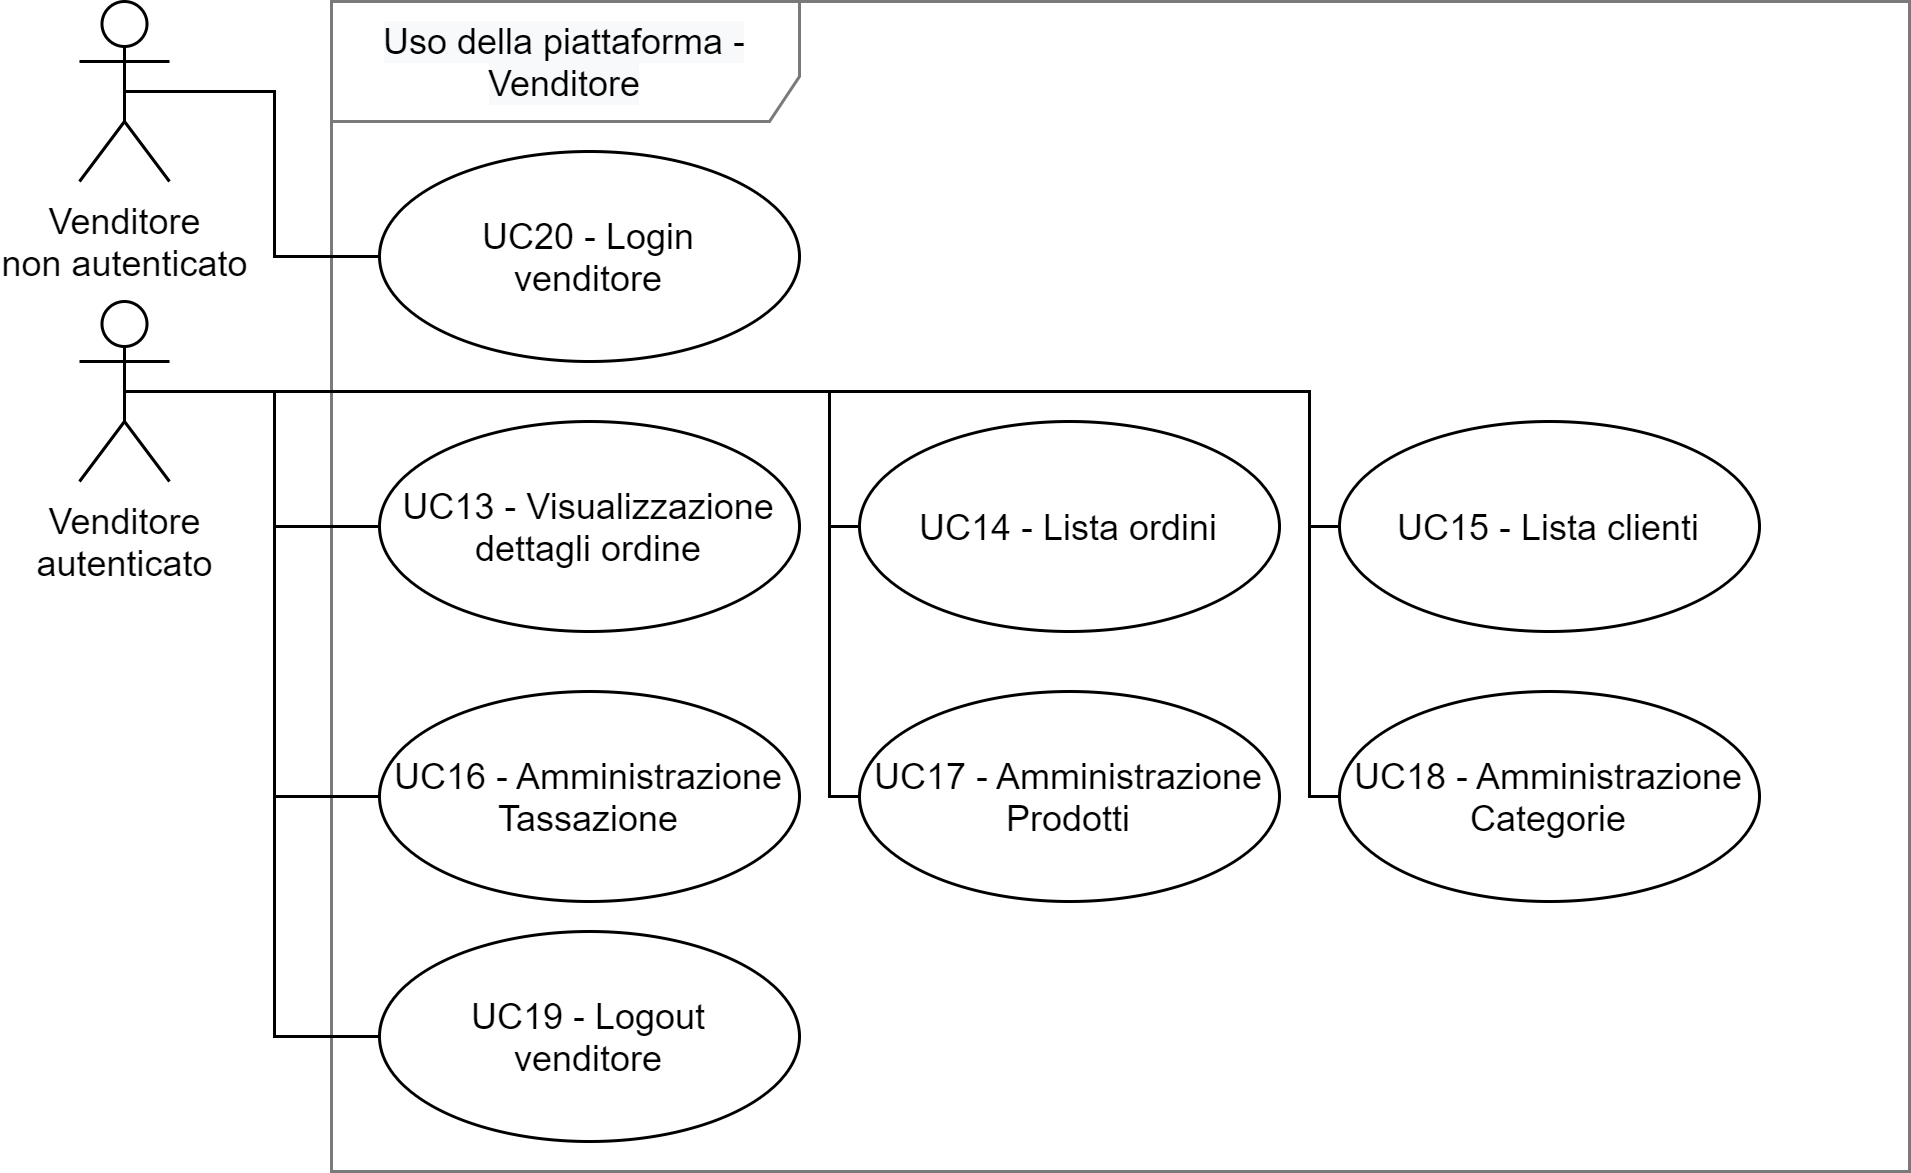
\includegraphics[width=\linewidth]{res/images/UC/venditore.png}
    \caption{Diagramma che descrive le funzionalità della piattaforma} 
\end{figure}

%contatore dei UserCases
\newcounter{CUC} % Contatore UserCases 
\newcounter{CSUC} % Contatore Sotto-UserCases
\newcounter{CSSUC} % Contatore Sotto-Sotto-UserCases
\newcommand{\stepUserCase}[0]{\stepcounter{CUC}\setcounter{CSUC}{0}\setcounter{CSSUC}{0}} % incrementa il contatore CUC
\newcommand{\stepsubUserCase}[0]{\stepcounter{CSUC}\setcounter{CSSUC}{0}} % incrementa il contatore CSUC
\newcommand{\stepsubsubUserCase}[0]{\stepcounter{CSSUC}} % incrementa il contatore CSSUC
\newcommand{\valueUserCase}[0]{UC\arabic{CUC} } % ritorna il valore del contatore CUC
\newcommand{\valuesubUserCase}[0]{UC\arabic{CUC}.\arabic{CSUC} } % ritorna il valore del contatore CSUC
\newcommand{\valuesubsubUserCase}[0]{UC\arabic{CUC}.\arabic{CSUC}.\arabic{CSSUC} } % ritorna il valore del contatore CSSUC
\newcommand{\resetCUC}[0]{\setcounter{CUC}{0}\setcounter{CSUC}{0}\setcounter{CSSUC}{0}}  % resetta il contatore CUC e CSUC
\newcommand{\labelUserCase}[0]{\label{UC\arabic{CUC}}}
\newcommand{\labelsubUserCase}[0]{\label{UC\arabic{CUC}.\arabic{CSUC}}}
\newcommand{\labelsubsubUserCase}[0]{\label{UC\arabic{CUC}.\arabic{CSUC}.\arabic{CSSUC}}}